\subsection{Experimento 1: Selección de Herramienta para la toma de Métricas de Consumo}\label{exp1-selecttool}
En esta primera fase de experimentación se han llevado a cabo una comparativa entre las diferentes herramientas disponibles para la toma de métricas de consumo sobre cargas de trabajo desplegadas en contenedores. Estas cargas de trabajo están basadas en la codificación de video y se llevarán a cabo empleando la herramienta \textbf{ffmpeg}.

Se ha utilizado un unico video compuesto por los chunks \textbf{18 a 43} del video \textbf{Skateboarding\_CableLabs}, debido a que el objetivo principal es determinar qué herramienta es capaz de tomar el conjunto de métricas de consumo más precisas.

El video resultante de la union de los chuncks, consta de una duración de 50 segundos con un CRF 0 a una resolución 4K(3840 x 2160) y con un bitrate de 1012693 kbps (1012,693 Mbps). Pese a que no es un video con una gran duración, tiene una gran calidad con 0 pérdida y un bitrate muy elevado, proporcionando sufiente carga de trabajo al codificador. Permitiendo extraer suficientes métricas  en un tiempo prolongado del proceso de codificación mediante CPU y GPU, ya que, por lo general, los códecs que utilizan la GPU para llevar a cabo la codificación son notablemente más rápidos que los codificadores que utilizan codificación únicamente sobre CPU.
\begin{lstlisting}[language=sh,label={code:exp1-ffmpeg-encoding},caption={Orden de codificación para codificadores CPU y codificadores GPU}]
#Codificación empleando CPU
docker exec ffmpeg-container ffmpeg -y -i /config/SkLab_3840x2160_crf0.mp4 -c:v [ libx264 | libx265 ] -b:v 4M -vf scale=1280:720 -c:a copy /config/output.mp4

 # Codificación empleando CPU+GPU
 docker exec ffmpeg-container ffmpeg -y -i /config/SkLab_3840x2160_crf0.mp4 -c:v [ h264_nvenc | hevc_nvenc ] -b:v 4M -vf scale=1280:720 -c:a copy /config/output.mp4
\end{lstlisting}


\subsubsection{Desarrollo de los experimentos de la primera fase}

 En total se han definido cuatro escenarios experimentales, cuyo objetivo es evaluar la capacidad de cada herramienta para recopilar métricas de consumo energético, así como el nivel de granularidad de la información obtenida. Para la ejecución de estos experimentos se ha desarrollado un conjunto de scripts en Bash, encargados de automatizar tanto el despliegue de las pruebas como la recopilación de las métricas generadas por cada herramienta. Cada escenario se ejecutará un total de diez veces y, entre conjunto de iteraciones consecutivas, se establecerá un intervalo mínimo de dos minutos. Este intervalo tiene como objetivo reducir la influencia que el estado térmico del sistema tras las ejecuciones anteriores pueda ejercer sobre las mediciones, así como minimizar las variaciones inherentes a la ejecución de las cargas de trabajo. De este modo, se pretende obtener resultados más representativos y consistentes.
 
 Los scripts empleados para realizar las pruebas con Kepler \ref{exp1:kepler-script-probes} y Scaphandre \ref{exp1:scp-script-probes} comparten una estructura común, adaptando únicamente el proceso de inicialización y la recopilación de métricas a las particularidades de cada herramienta. En ambos casos es necesario especificar la ruta del vídeo que será codificado, el nombre del contenedor encargado de ejecutar el proceso de codificación y el directorio en el que se almacenarán las métricas obtenidas.
 
 Por otra parte, los scripts desarrollados para la herramienta Container Energy Monitoring \ref{exp1:monitor-script-probes-1container} y \ref{exp1:monitor-script-probes-2containers} requieren una configuración ligeramente más detallada. Además de indicar el contenedor que ejecutará la codificación y el directorio de salida de los resultados, es necesario definir el nombre del experimento, el número de iteraciones que se realizarán y el nombre de los archivos en los que se almacenarán las métricas recopiladas durante cada ejecución.
 
 Cabe destacar que, en el caso de Container Energy Meter, se han empleado dos scripts con el fin de evitar perder más tiempo y poder proseguir con la fase experimental 2, y poder cumplir con los plazos de entrega. Ambos scripts son prácticamente el mismo, a diferencia de \ref{exp1:monitor-script-probes-2containers} el cual lleva a cabo las acciones del script \ref{exp1:monitor-script-probes-1container} dos veces, almacenando los datos resultantes de la recolección en archivos diferenciados.


\subsection{Post-procesamiendo de las Métricas de Consumo Energético}
 Una vez finalizada la fase de experimentación, el procesamiento de los datos obtenidos en cada iteración se llevará a cabo mediante un nuevo conjunto de scripts desarrollados en Bash. Estos scripts se encargan de procesar las métricas recopiladas en cada ejecución, calcular el valor medio para cada escenario experimental y almacenar los resultados en un archivo CSV.
 
 En el caso de Kepler \ref{exp1:kepler-data-procesor} y Scaphandre \ref{exp1:scp-data-procesor}, el archivo CSV se genera en el mismo directorio donde se encuentran almacenados los datos de cada iteración. Por el contrario, la herramienta Container Energy Monitoring almacena el archivo resultante en un directorio denominado \texttt{data}. En todos los casos es necesario indicar la ruta donde se encuentran los datos que se desean procesar, así como el nombre del archivo CSV de salida.
 
 Aunque los archivos CSV generados por cada herramienta presentan una nomenclatura diferente, todos ellos contienen información equivalente relativa a las métricas de consumo energético recopiladas durante la experimentación. En las siguientes figuras se muestra un ejemplo de la cabecera generada por cada herramienta:

 \begin{figure}[h!]
      \centering
 	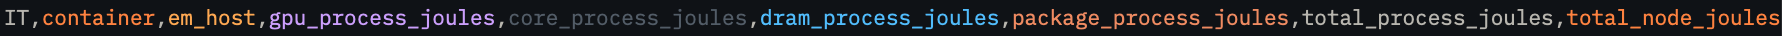
\includegraphics[width=\linewidth]{figs/exp1_kepler_csv_header.png}  
 	\caption{Header CSV del archivo de datos procesados de Kepler}  
 	\label{fig:exp1-kepeler-csv_header}
 \end{figure}
 
 \begin{figure}[h!]
      \centering
 	
\includegraphics[width=\linewidth]{figs/exp1_scp_csv_header.png}  
 	\caption{Header CSV del archivo de datos procesados de Scaphandre}  
 	\label{fig:exp1-scp-csv_header}
 \end{figure}
 
 \begin{figure}[h!]
 \centering
 	
\includegraphics[width=\linewidth]{figs/exp1_monitor_csv_header.png}  
 	\caption{Header CSV del archivo de datos procesados de Container Energy Monitoring}  
 	\label{fig:exp1-monitor-csv_header}
 \end{figure}

Finalmente, para generar las tablas y gráficas comparativas entre las distintas herramientas en cada escenario experimental, se ha desarrollado un script en Python \ref{exp1:python-bar-grafics}. Este script procesa los archivos CSV generados por cada herramienta, calcula las métricas agregadas necesarias para el análisis comparativo y almacena los resultados en un nuevo archivo CSV. Dicho archivo constituye la entrada para la generación de las gráficas de barras histográficas y tablas comparativas que se presentan en el capítulo de resultados. 

A continuacion se detalla una lista de los posibles valores y su representación en la siguiente lista:
\begin{itemize} 
 \item \texttt{em\_total\_energy}: Energia total del sistema calculada en base añ consumo energetico de los grupos de comonentes $PKG+DRAM$ de RAPL estimada por Global Energy Meter. 
 \item \texttt{node\_total\_joules}: Energia total del sistema estimada por la herramient.
 \item \texttt{process$N$\_energy\_joules}: Energia total consumida por el proceso de transcodificacion $N$ estimado por la herramineta y ejecutado sobre el contenedor con \textit{FFMPEG}.  
 \item \texttt{gpu\_node\_jouls}: Energia consumida por la GPU durante el proceso de codificación estimado por la herramienta.
 \end{itemize}

\subsection{Analisis de resultante la sección Experimento 1}

\subsubsection{Escenario 1: Transcodificacion empleando un contenedor unicamente con CPU}
 En el siguiente escenario, se ha llevado a cabo la transcodificación de video sobre un contenedor utilizando un codificador basado CPU(\textit{x264} o \textit{x265}), cuyos resultados pueden apreciarse en la siguiente grafica de histogramas \ref{fig:exp1-es2-resultados}. 

 En relación a las métricas de consumo del nodo respecto a la metrics recolectadas por Global Energy Meter, se observa que la herramieta con menor discrepancia es \textbf{Global Energy Container}, con una tasa de error del \textbf{$0,3113\%$}. Seguido por \textbf{Scaphandre} con un \textbf{$3,4955\%$} y Kepler con un \textbf{$4,6850\%$}. 
 
 Estos resultado muestran como la capacidad para tomar métricas de consumo de un unico proceso ejecutado sobre un contenedor tiene mayor precision que \textit{Kepler} y a \textit{Scaphandre}.

 \begin{figure}[h!]
    \centering
    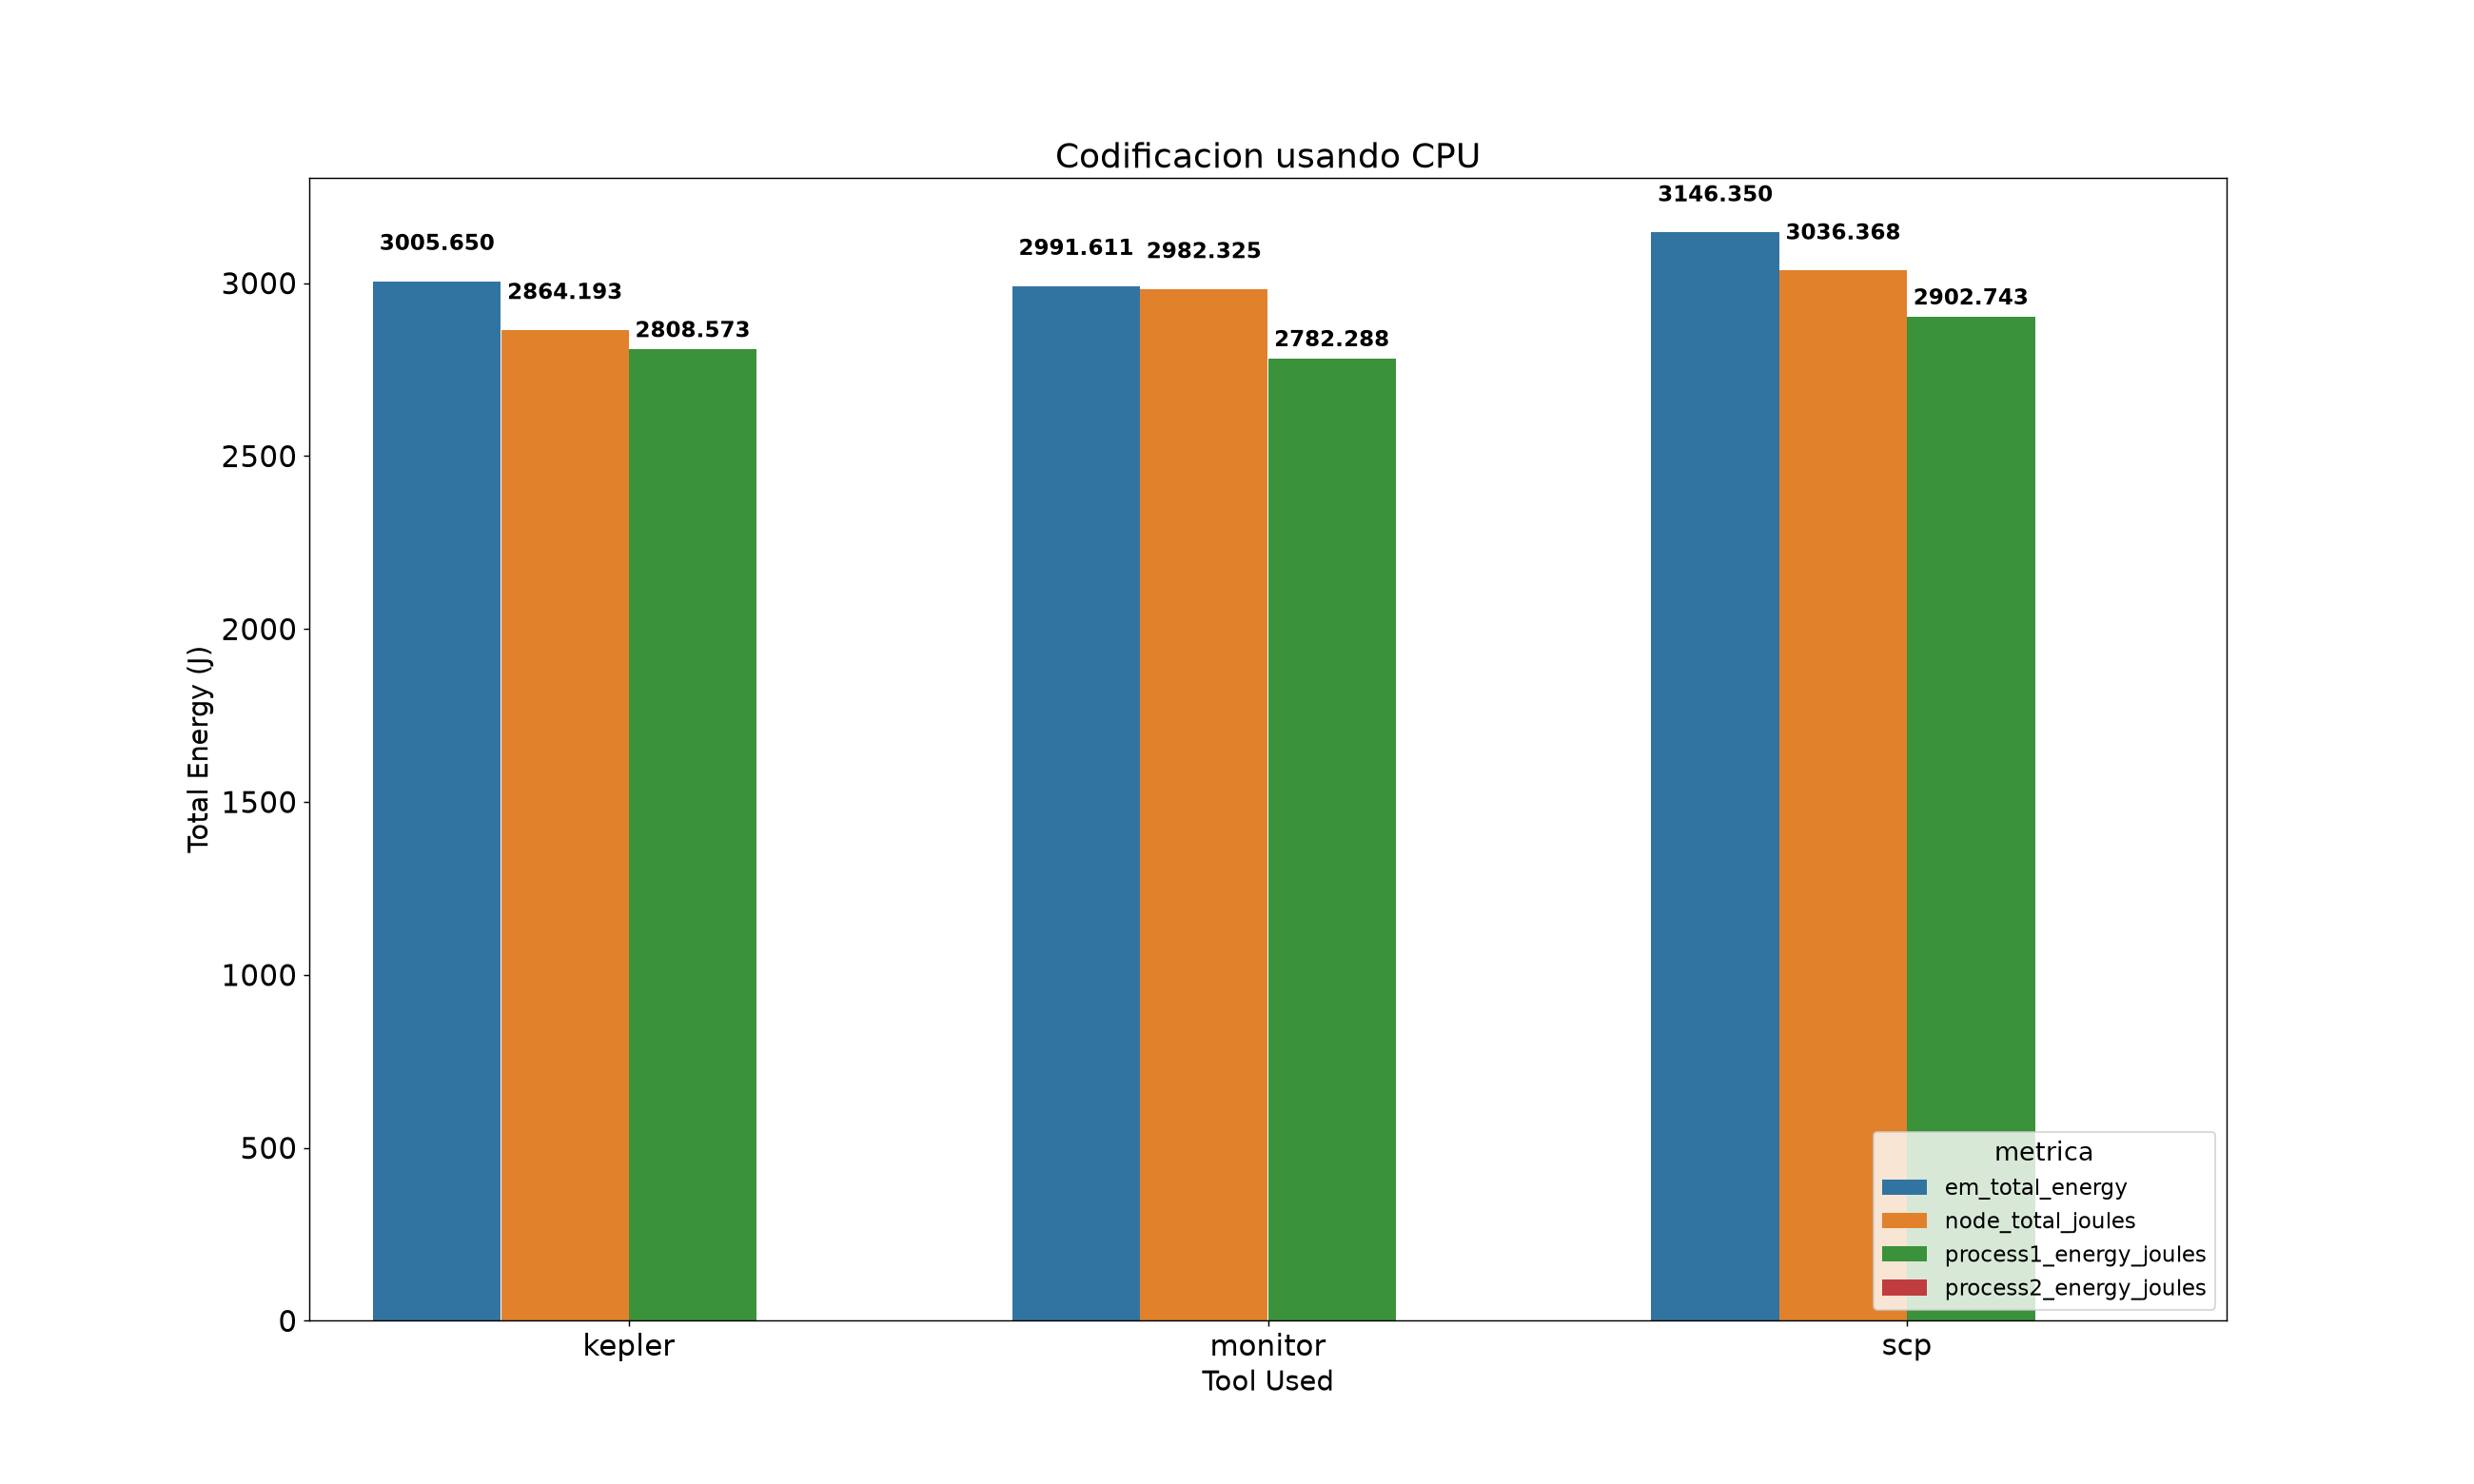
\includegraphics[width=\linewidth]{figs/exp1-1cont-nolimit.png}
    \caption{Histograma comparativo de las métricas de consumo energetico en julios de las tres herramientas sobre una tarea de transcodificacion llevada a cabo en un contenedore de docker (process1\_energy\_joules)}
    \label{fig:exp1-es2-resultados}
 \end{figure}

\subsubsection{Escenario 2: Transcodificación sobre un contenedor empleando CPU y GPU}
  En este escenario se le da acceso al contenedor tanto a la GPU como al numero total de cores de la CPU. Con esta comparativa se espera poder medir las capacidades basicas de cada una de las herramientas al tratar de determinar el consumo del nodo y de la GPU, asi como del proceso que se estan ejecutando sobre este en comparacion a las métricas de energia recolectadas por la herramienta externa Global Energy Meter.
  
  Cabe destacar que la energía total medida por \textit{Global Energy Meter} (\textbf{em\_total\_energy}) y por las herramientas de métricas respecto al nodo (\textbf{node\_total\_joules}) miden el consumo energético basándose en RAPL, lo cual implica que ninguna de estas medidas incluye el consumo de la tarjeta gráfica. Por tanto, para conocer el consumo total del sistema durante el proceso de codificación empleando tarjeta gráfica, se deben sumar las métricas de consumo del nodo y la métrica de consumo de la GPU (\textbf{gpu\_node\_jouls}) \(\textbf{gpu\_node\_jouls}+\textbf{em\_total\_energy} = \textbf{Total\_Energy\_System}\).
 
  En cuanto a la capacidad de tomar métricas de las herramientas, se observa que Scaphandre es la única herramienta que no ha sido capaz de tomar métricas de consumo energético de la GPU. En cambio, tanto Kepler como Container Energy Monitoring sí que han sido capaces de medir el consumo energético, siendo en ambos casos bastante similares. Esto nos sirve de indicativo de que el hotfix realizado sobre Kepler se comporta segun la referencia de consumo esperada, ademas de indicar que la capacidad de tomar métricas de consumo de la tarjeta gráfica de ambas herramientas parece ser adecuada.
 
  Si nos centramos en la capacidad para medir el consumo energético del nodo, Container Energy Monitoring es la que menor discrepancia presenta respecto a la energía que Global Energy Meter ha tomado del sistema, con una tasa de error del \textbf{$0,41\%$} calculada empleando la formula \ref{eq:percent-energy-node}. Seguida por Scaphandre quien presenta una tasa de error del 	\textbf{$3,06\%$}, y , en ultimo lugar, Kepler quien presenta un tasa de error del \textbf{$7,45\%$}.
 
  \begin{figure}[h!]
     \centering
     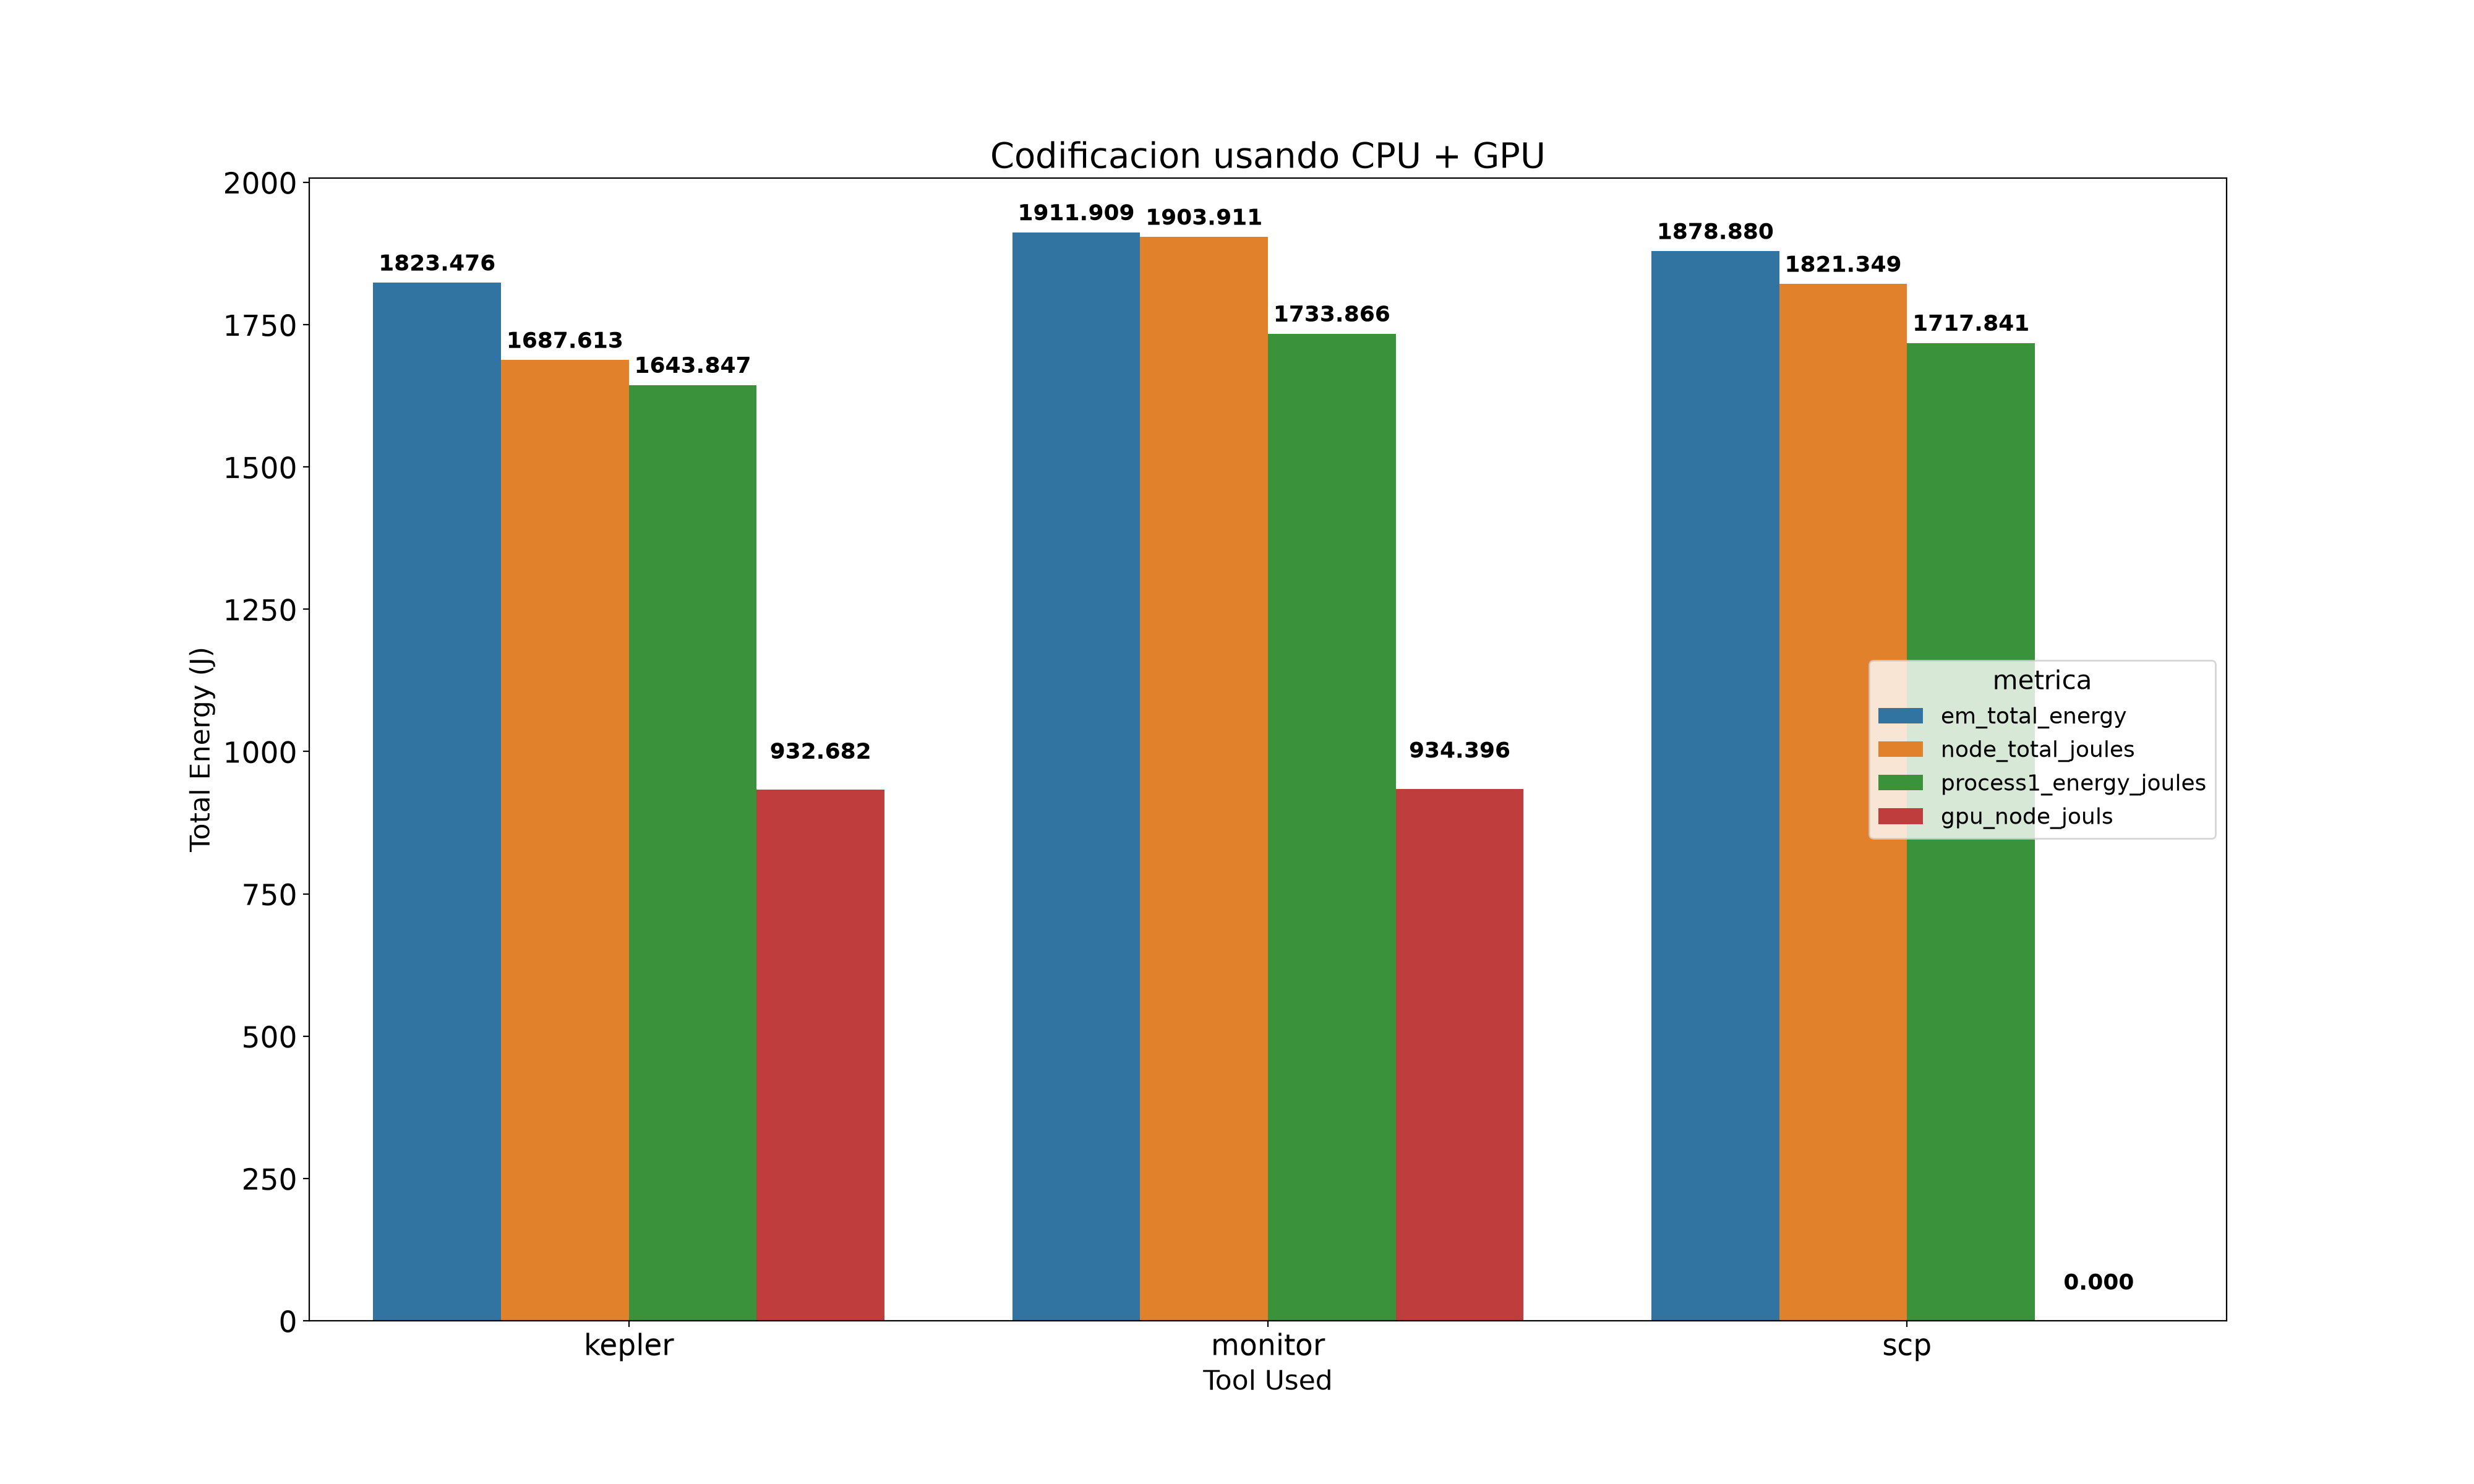
\includegraphics[width=\linewidth]{figs/exp1-1cont-nolimitcpuygpu.png}
     \caption{Histograma resultante de las métricas de consumo energetico en julios sobre una tarea de codificación empleando GPU y CPU}
     \label{fig:exp1-es1-resultados}
  \end{figure}


\subsubsection{Escenario 3: Transcodificacion empleando un contenedor limitado a tres cores}
 En este tercer escenario, se ha limitado el numero de cores a los que el contenedor tiene acceso con el fin de medir la granularidad de cada una de las herramientas en relacion a las métricas de consumo. Para limitar el numero de cores se han añadido las opciones:
 \begin{itemize} 
  \item \texttt{\lstinline[language=sh]{--cpus="3"}}: Numero de cores que el contenedor puede utilizar.
  \item \texttt{\lstinline[language=sh]{--cpuset-cpus=1-3}}: Rango de las cores de las que dispone, en este caso reservamos los cores \textit{0,4,5,6 y 7} para el sistema.
 \end{itemize}
 
 Analizando el consumo energetico general de las diferentes métricas, se observa un aumento del consumo energetico del \textbf{$31,99\%$} respecto al escenario que no presentaba limitacion en el numero de cores de la CPU. En cuanto a la metrica de consumo energetico del nodo, Container Energy Monitoring es el que menor discrepancia tiene respecto a la energia medida por Global Energy Meter con una tasa de error del \textbf{$0,2546\%$}. Seguido por Scaphandre, quien presenta un tasa de error del \textbf{$2,5921\%$} respecto a la energia medida por Global Energy Meter, y en ultimo lugar, Kepler el cual presenta un tasa de error del \textbf{$62,5930\%$}, una gran diferencia respecto tasa de error de las dos herramientas.
 
 Los resultados muestran que Container Energy Monitor es la herramienta que mejor atribuye la energía en el caso se que limite el número de cores asignados al contenedor. En este mismo escenario, Kepler y Scaphandre dan un valor muy bajo a la energía consumida por el contenedor. Para determinar las causas habría que analizar el código fuente, lo que queda fuera del ámbito de este trabajo.

 \begin{figure}[h!]
   \centering
   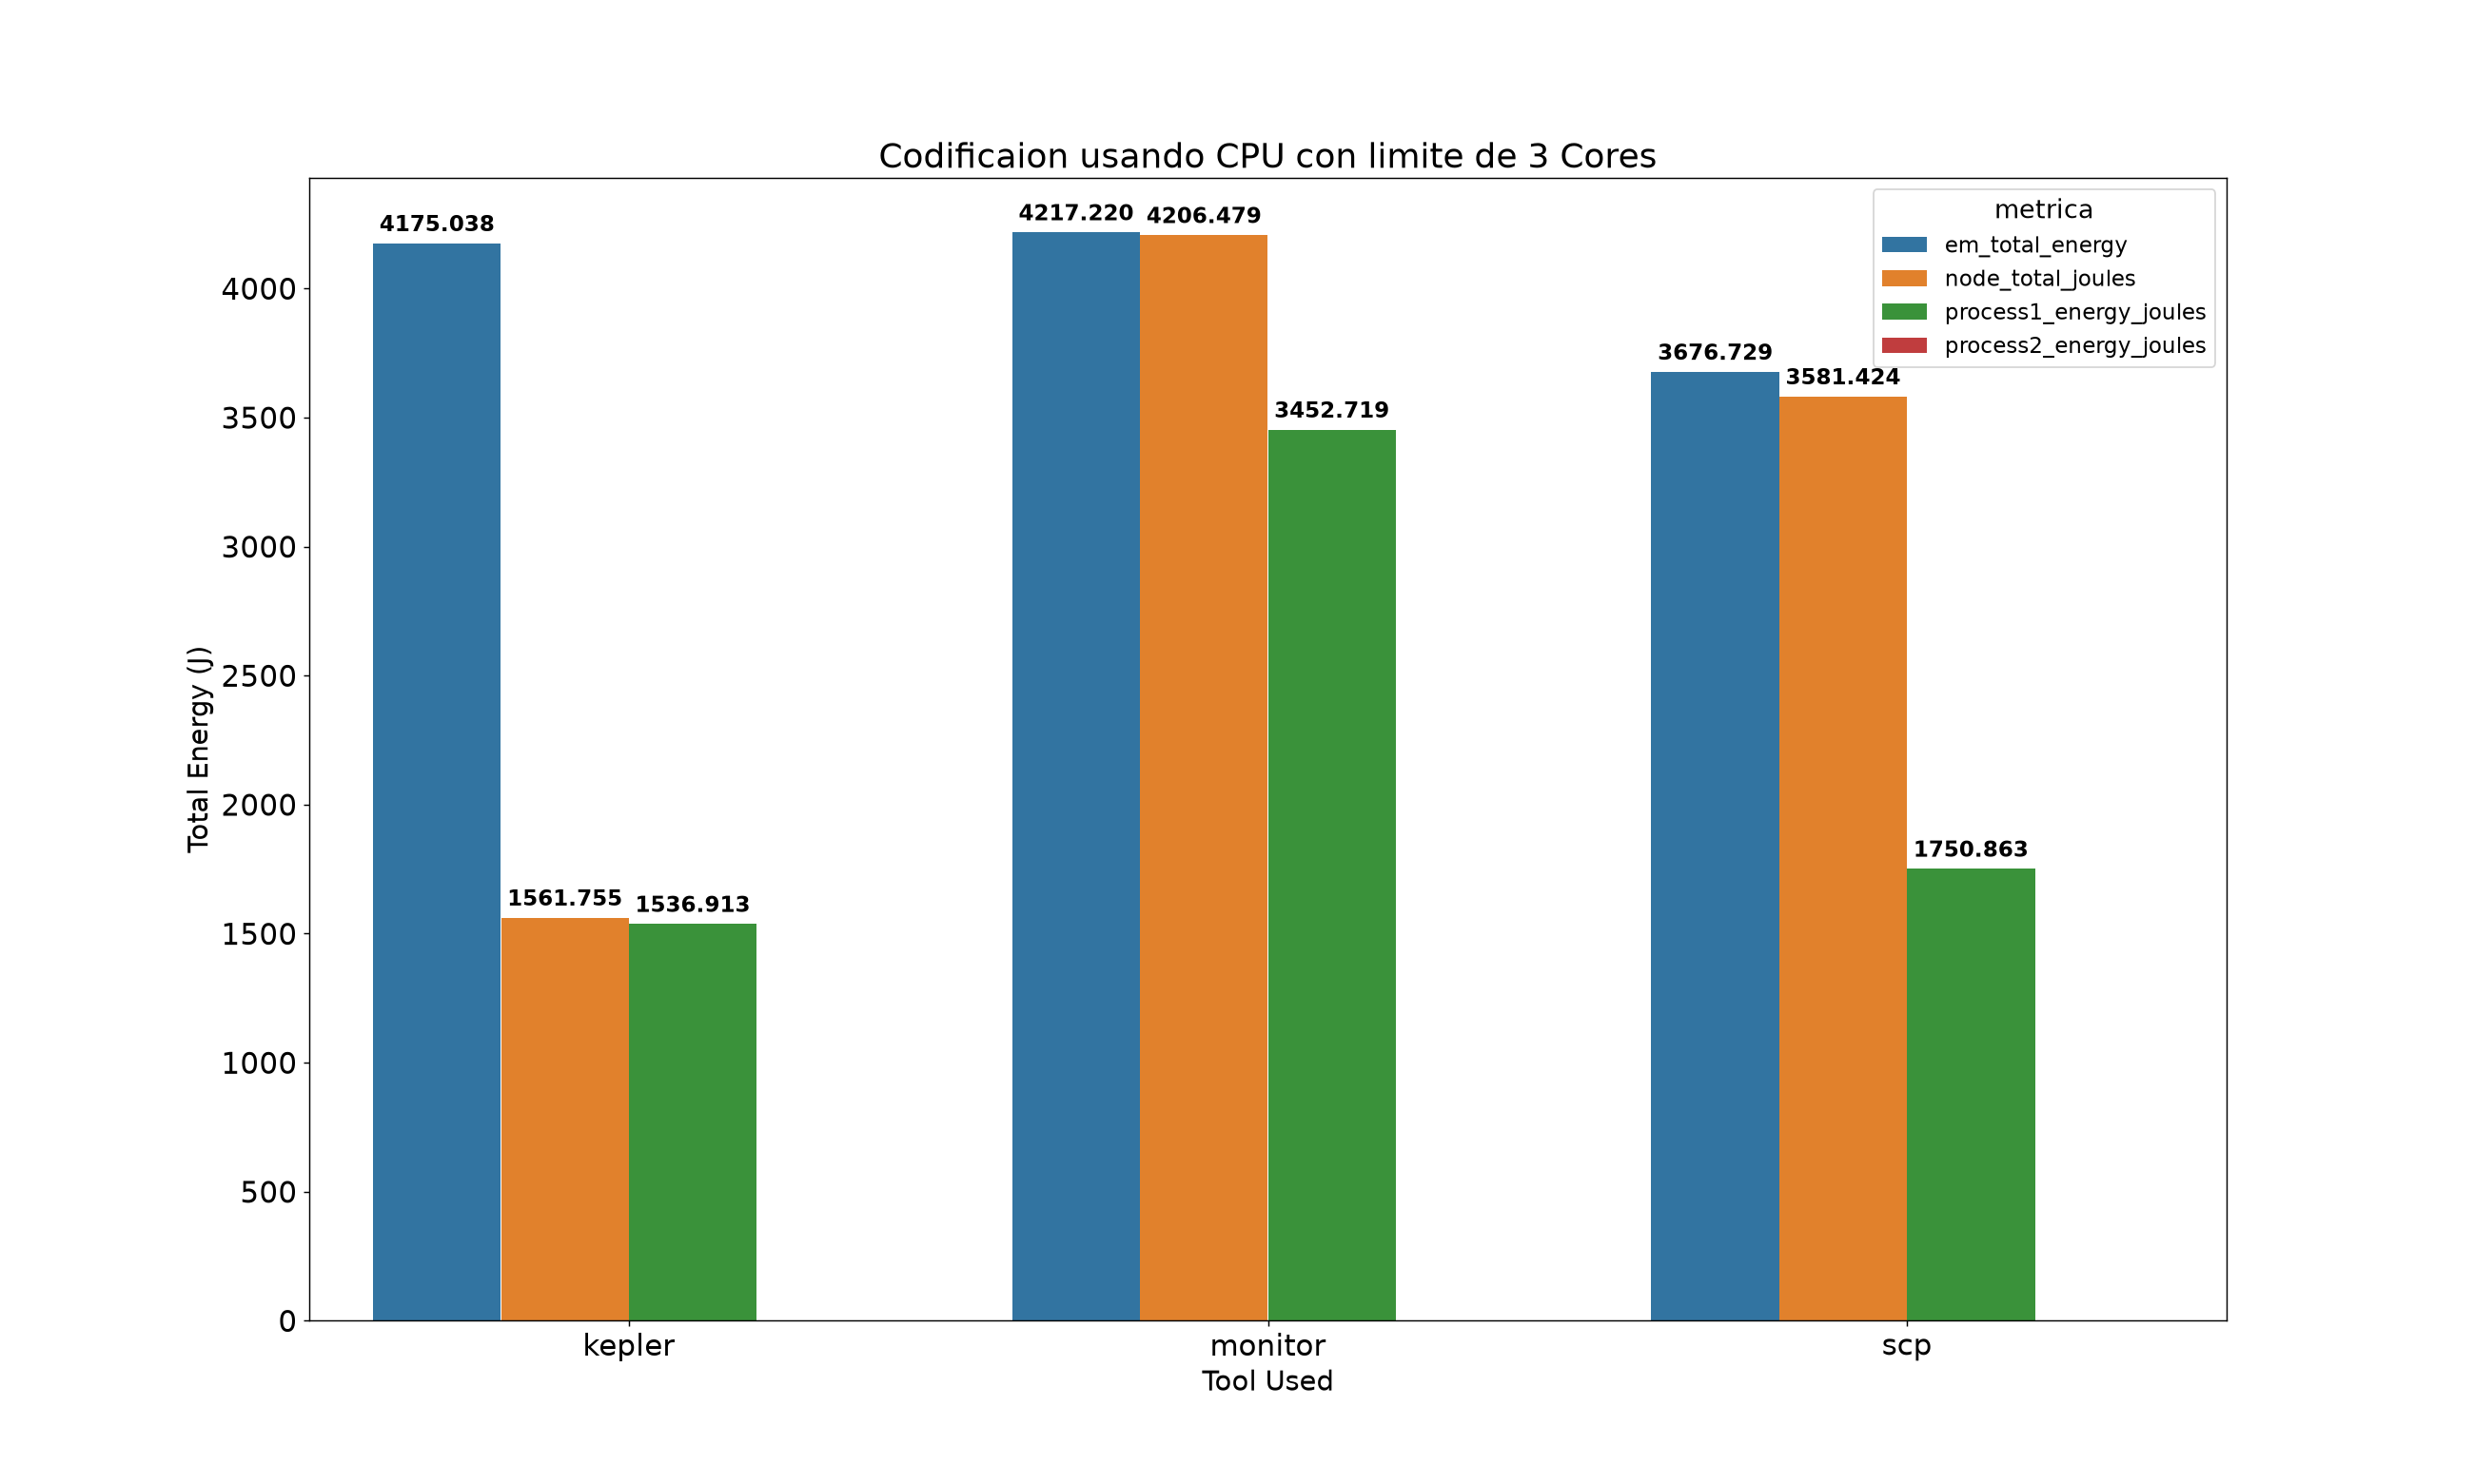
\includegraphics[width=\linewidth]{figs/exp1-1cont-limited3cpus.png}
   \caption{Histograma resultante delas métricas de consumo sobre una tarea de codificacion emplendo un contenedor limitado a 3 cores}
   \label{fig:exp1-es3-resultados}
 \end{figure}

\subsubsection{Escenario 4: Transcodificacion concurrente empleando dos contenedores limitados a tres cores cada uno}
 Finalmente, en el cuarto escenario experimental se limita el acceso a los recursos disponibles, distribuyendo la carga de trabajo entre dos contenedores. A cada contenedor se le asignan tres núcleos de CPU, reservando nuevamente los núcleos 0 y 7 para el sistema operativo. De este modo, el primer contenedor utiliza los núcleos 1--3, mientras que el segundo utiliza los núcleos \textit{4--6}. En este escenario, se van a usar el codificador que usa exclusivamente la CPU.
 
 En esta última fase se pretende evaluar la precisión y granularidad de las herramientas al monitorizar de forma simultánea el consumo energético asociado a dos contenedores que ejecutan procesos de transcodificación independientes. Los resultados obtenidos se muestran en la Figura \ref{fig:exp1-es4-resultados}.
 
 En relación a la estimacion de consumo energético respecto a la energia del nodo, \textbf{Container Energy Monitoring} presenta los resultados más próximos a la referencia obtenida mediante Global Energy Meter, con una tasa de error del \textbf{$0,5428\%$}. Seguido de Scaphandre, cuya medición presenta una diferencia de aproximadamente \textbf{200-300 julios}, lo que supone una tasa de error del \textbf{$2,9988\%$}, respecto a dicha referencia. En el caso de Kepler, se observa una discrepancia considerable en la estimación del consumo energético del nodo, con una tasa de error del \textbf{$25,1623\%$}. 
 
 Si se analiza específicamente el consumo energético atribuido a a los dos procesos de transcodificación, \textbf{Scaphandre} proporciona una estimación total de \textbf{$4653,025$ julios}. Por otro lado, el consumo energético medido por  Global Energy Meter asciende a \textbf{$6815,315$ julios}. Por tanto, se calcula \ref{eq:percent-energy-tool_node} que el consumo atribuido a los procesos representa aproximadamente el \textbf{$68,2730\%$} del consumo total estimado para el nodo. Es decir, las dos cargas principales de trabajo son los procesos de codificación y según esta herramienta un \textbf{30\%} de la energía (unos $2\,000$ julios) no se atribuye a estos procesos.
 
 Por su parte, Container Energy Monitoring proporciona una estimación del consumo energético asociado a los procesos cuya suma asciende a \textbf{$6212,860$ julios}, frente a un consumo energético medido por  Global Energy Meter de \textbf{$6733,879$ julios}. Esto supone una diferencia de \textbf{$521,019$ julios} y significa que \textbf{Container Energy Monitoring} atribuye aproximadamente el \textbf{$92,2627\%$} del consumo energético total del nodo a los procesos ejecutados en los dos contenedores. Este resultado es coherente con las condiciones del escenario descrito anteriormente, en el que la mayor parte de la carga de trabajo del sistema corresponde a los procesos de transcodificación ejecutados simultáneamente en ambos contenedores.

 En el el caso de la métricas tomadas por \textbf{Kepler}, se obtiene que ambos procesos han consumido un total de $4943,986$ julios mientras que Global Energy Meter indica que el nodo ha consumido $6694,905$ julios. Esto implica que kepler atribuye un \textbf{$73,8469\%$} de energia a los procesos de transcodificación. Esto implica que segun esta herramienta un \textbf{$26,19\%$} de la energia no se asigna a ningun proceso.


 \begin{figure}[h!]
     \centering
     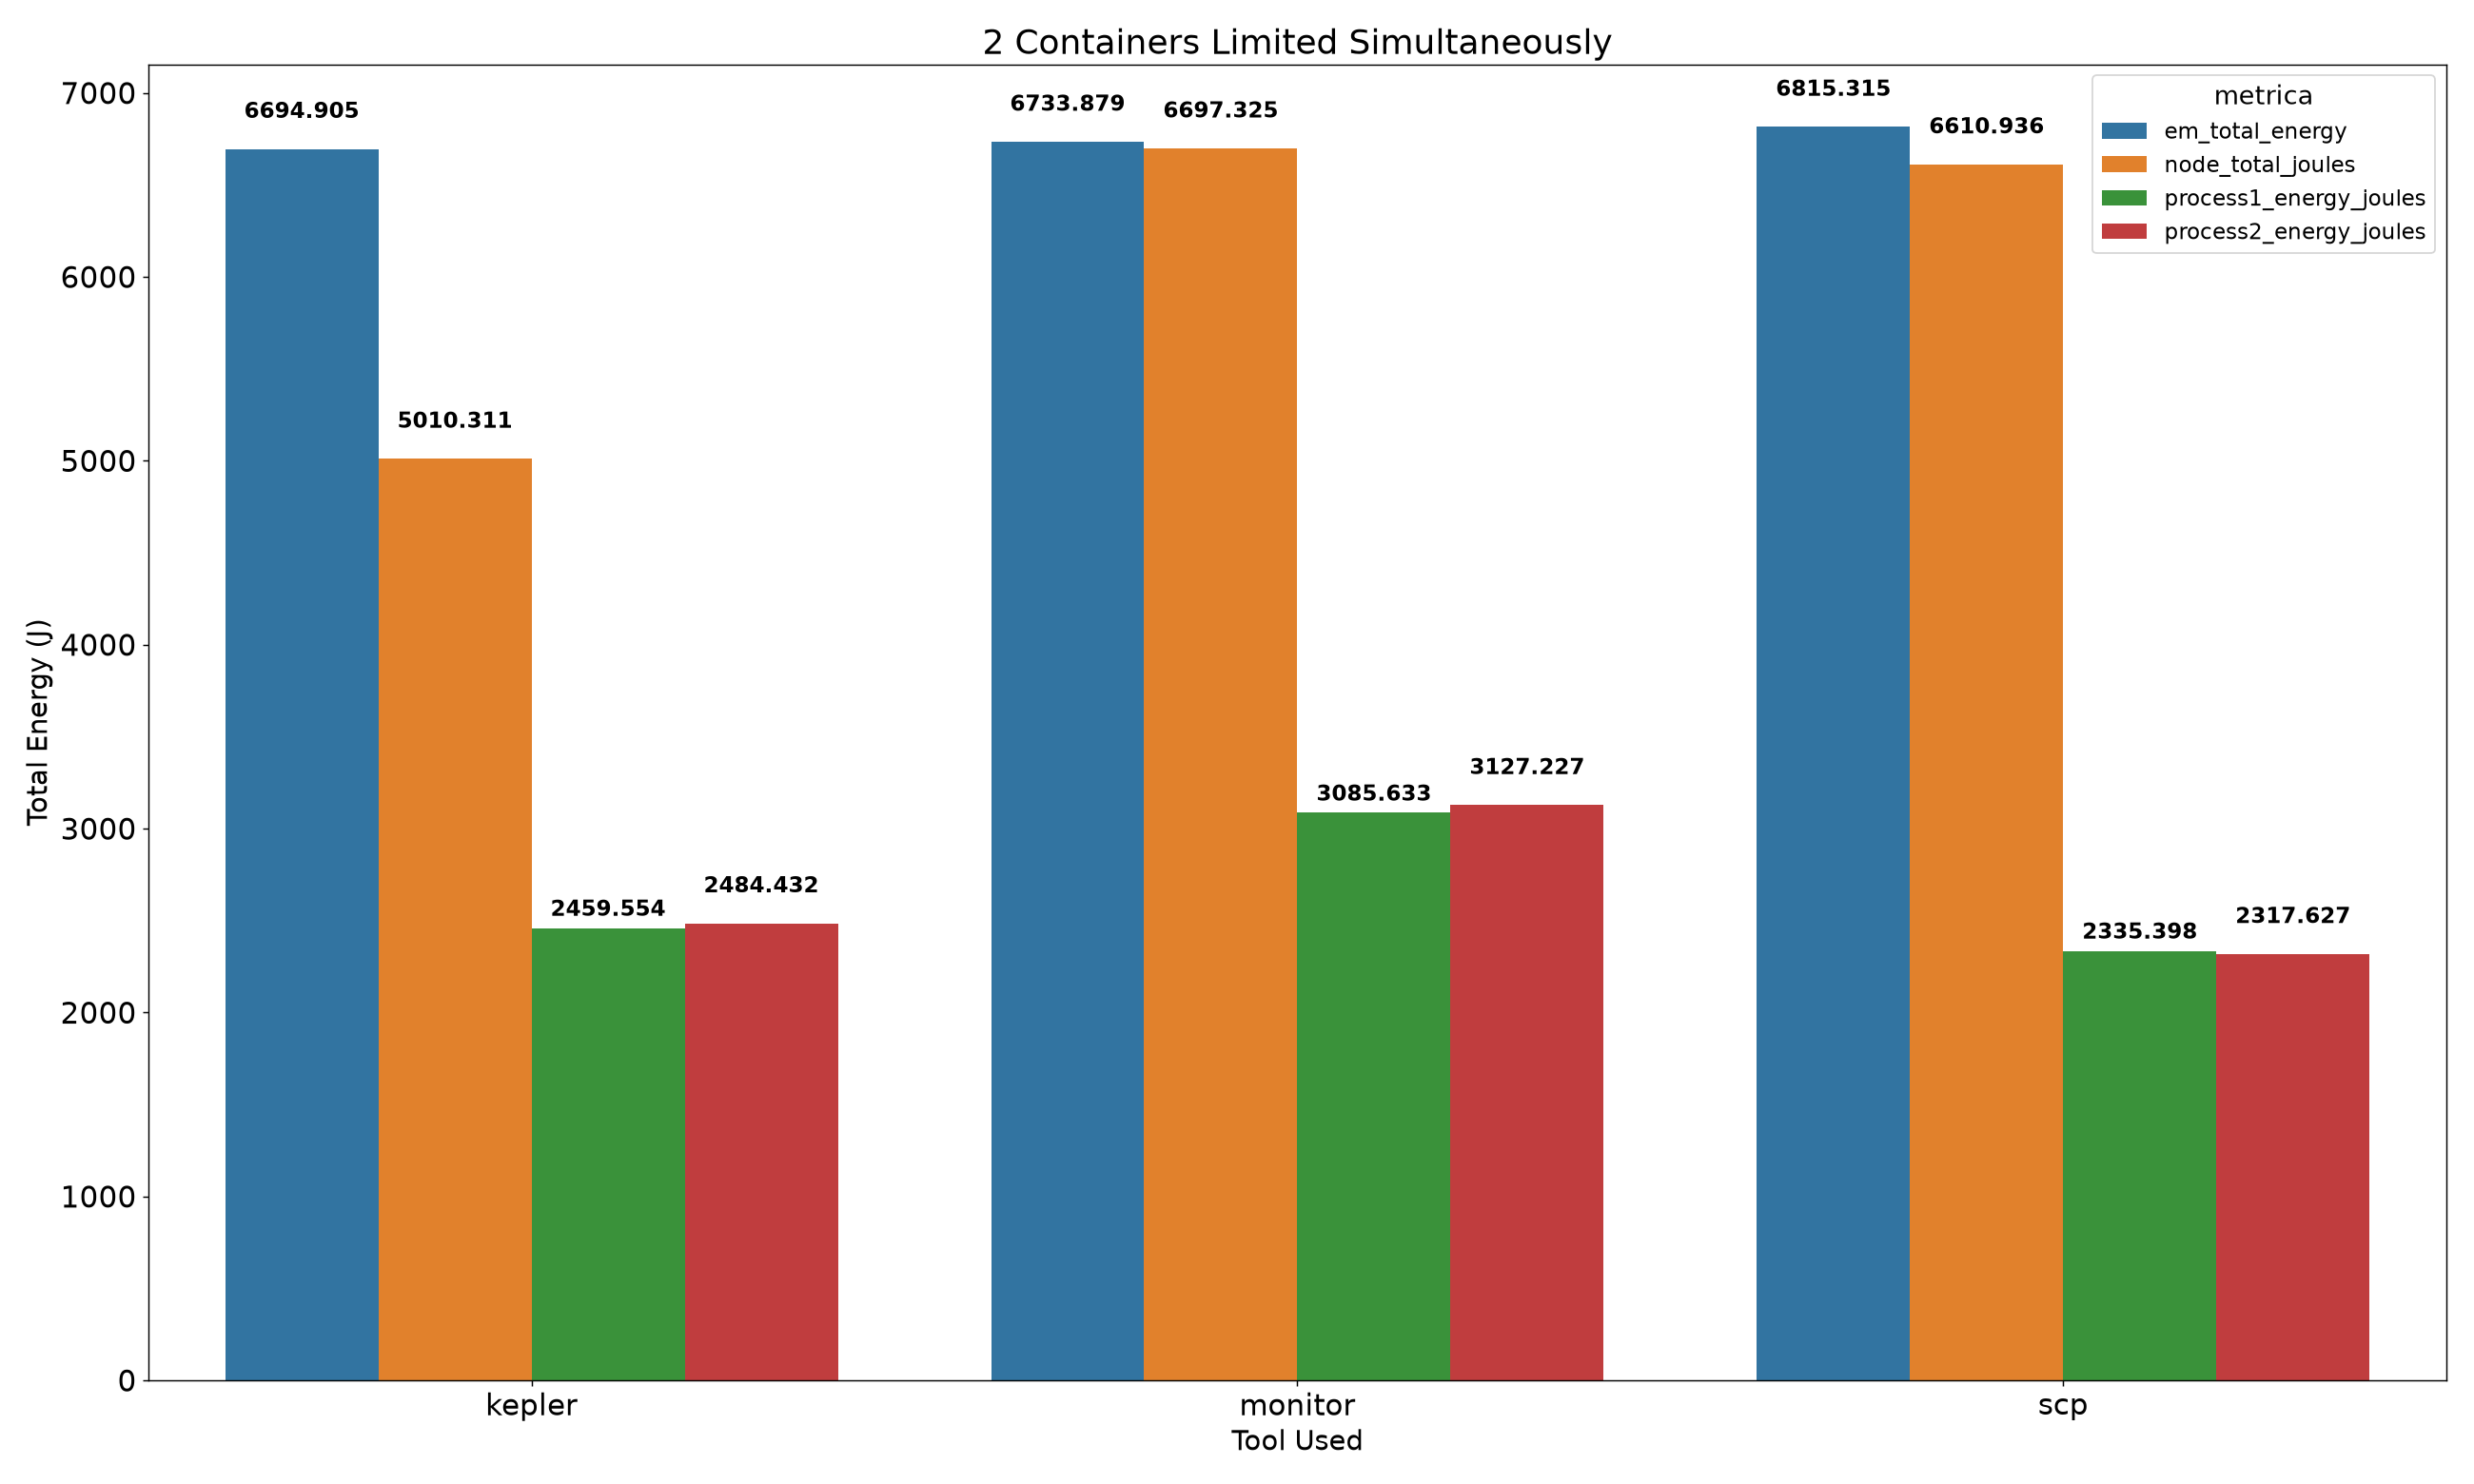
\includegraphics[width=\linewidth]{figs/exp1-2cont-limited3cpus.png}
     \caption{Histograma resultante de las métricas de consumo de dos contenedores limitados a 3 cores cada uno ejecutando tareas de codificacion simultaneamente}
     \label{fig:exp1-es4-resultados}
 \end{figure}

\subsection{Conclusiones fase 1 de la experimentacion }

Los experimentos llevados a cabo en esta primera fase han permitido comparar el comportamiento de \textit{Scaphandre}, \textit{Kepler} y \textit{Container Energy Monitoring} bajo distintas condiciones de ejecución, teniendo en cuenta tanto el consumo energético total del nodo como la posibilidad de atribuir dicho consumo a los procesos monitorizados. Los resultados obtenidos muestran diferencias importantes entre las herramientas, especialmente en situaciones donde se limitan diferentes recursos del sistema y se varía la carga de trabajo e incluso el número de procesos que se ejecutan al mismo tiempo.

En cuanto a la estimación del consumo energético del nodo, \textit{Container Energy Monitoring} es el que menor discrepancia respecto a la medida de referencia utilizada presenta, de forma general. En los escenarios estudiados, los errores obtenidos por esta herramienta se mantienen en valores bajos, llegando a un error del \textbf{0.25\%} en el escenario 3 y un error del \textbf{0.31\%} en el escenario 2. Scaphandre también da estimaciones cercanas a las de referencia en algunos casos, pero tiene mayor diferencia en el escenario 4. Por su parte, Kepler presenta un comportamiento más variable, alcanzando un error del \textbf{62.59\%} en el escenario 3.

Además de la estimación del consumo del nodo, la capacidad de desagregar el consumo entre las cargas de trabajo constituye un aspecto especialmente relevante para los objetivos de este trabajo. En este sentido, \textbf{Container Energy Monitoring} presenta una mayor capacidad de atribución del consumo energético a los procesos monitorizados. Esto resulta especialmente significativo en el escenario 4, donde consigue atribuir a los procesos el \textbf{92.77\%} del consumo total medido para el nodo, frente al \textbf{70.40\%} obtenido por Scaphandre y el \textbf{22.37\%} obtenido por Kepler. Por tanto, Contanier Energy Meter es la herramienta que mejor consigue estimar la energía en un escenario donde hay concurrencia de procesos y los contenedores tienen recursos limitados.

\begin{table}[htbp]
     \centering
     \begin{tabularx}{\textwidth}{|>{\raggedright\arraybackslash}X|r|r|r|}
     \hline
     \rowcolor[HTML]{C0C0C0} 
     Herramienta & \multicolumn{1}{c|}{GEM (j)} & \multicolumn{1}{c|}{Energia del Procesos (j)} & \multicolumn{1}{c|}{Energía Sin Atribuir (\%)} \\ \hline
     Global Energy Monitor & 6733,879 & 6212,860 & 7,73 \\ \hline
     Scaphandre & 6815,315 & 4653,025 & 31,73 \\ \hline
     Kepler & 6694,905 & 4940,98 & 26,19 \\ \hline
     \end{tabularx}
     \caption{Tabla comparativa de las métricas de consumo de los procesos de codificación obtenidos por cada herramienta, junto con el porcentaje de energía sin atribuir frente a la energía medida en cada caso por Global Energy Meter.}
     \label{tab:exp1-conclusiones-esc4}
\end{table}

Por otra parte, los resultados alcanzados posibilitan la identificación de ciertas limitaciones de las herramientas evaluadas. Scaphandre tiene ciertas limitaciones a la hora de obtener información energética relacionada con algunos recursos de hardware, como la GPU. También tiene limitación a la hora de tomar métricas sobre múltiples procesos sobre múltiples contenedores en simultáneo, ya que, como se puede observar en la tabla comparativa \ref{tab:exp1-conclusiones-error}, el error respecto a la energía medida por EM escala conforme al número de procesos aumenta.  

En el caso de Kepler, si bien no tiene problemas para medir el consumo sobre la GPU, presenta discrepancias importantes a la hora de estimar el consumo energético del nodo, con un gran nivel de error, lo que restringe su elección como herramienta de toma de métricas de uno o varios procesos del sistema. Este factor dificulta la posibilidad de saber si las métricas recolectadas del conjunto de procesos están sobreestimadas o, por el contrario, muy por debajo del consumo real.

Estas diferencias muestran que es importante seleccionar la herramienta no solo por su capacidad de obtener una medida energética, sino también por la granularidad y nivel de atribución que ofrece.

Por lo tanto, y teniendo en cuenta la discrepancia respecto a la referencia, la capacidad de atribución del consumo a los procesos y el comportamiento observado en los distintos escenarios, se selecciona Container Energy Monitoring como herramienta para las siguientes fases del estudio. Esta selección facilitará una mayor precisión en la medición del consumo energético de las cargas de trabajo implementadas, elemento clave para posteriormente examinar el impacto energético de los diferentes escenarios de transcodificación estudiados en este trabajo.

\begin{table}[ht!]
     \centering
     \begin{tabularx}{\textwidth}{|>{\raggedright\arraybackslash}X|r|r|r|r|}
     \hline
     \rowcolor[HTML]{C0C0C0} 
     Herramientas & ES1 & ES2 & ES3 & ES4 \\ \hline
     \cellcolor[HTML]{EFEFEF}KEPLER & $4,685\%$ & $7,45\%$ & $62,593\%$ & $25,16\%$ \\ \hline
     \cellcolor[HTML]{EFEFEF}SCP & $3,4955\%$ & $3,06\%$ & $2,5921\%$ & $2,9988\%$ \\ \hline
     \cellcolor[HTML]{EFEFEF}Container Energy Monitor & $0,3113\%$ & $0,41\%$ & $0,2546\%$ & $0,5428\%$ \\ \hline
     \end{tabularx}
     \caption{Tasa de error de estimación de consumo energético en el nodo en comparación con la energía medida por Global Energy Meter en cada uno de los escenarios}
     \label{tab:exp1-conclusiones-error}
\end{table}

